\documentclass[a4paper,12pt]{article}

\usepackage[perpage]{footmisc}
%\setlength{\bibsep}{0.0pt}
%% Sets page size and margins
\usepackage[a4paper,top=3.cm,bottom=3.cm,left=2.4cm,right=2.4cm,marginparwidth=1.75cm]{geometry}


\usepackage{color}
\newcommand{\todo}[1]{\textcolor{red}{ #1}}
\newcommand{\toimprove}[1]{\textcolor{orange}{ #1}}
\newcommand{\mg}[1]{\textcolor{green}{MG: #1}}
\newcommand{\md}[1]{\textcolor{pink}{MD: #1}}
\newcommand{\sk}[1]{\textcolor{blue}{SK: #1}}
\newcommand{\cng}[1]{\textcolor{red}{#1}}

\usepackage[autolanguage,np]{numprint}

\usepackage{booktabs} % For formal tables

\usepackage{algorithm}
\usepackage[noend]{algpseudocode}
\usepackage{hyperref}
\usepackage[utf8]{inputenc}

\usepackage{siunitx}
\usepackage[autolanguage,np]{numprint}
\usepackage[toc,page]{appendix}

\usepackage{multirow}
\usepackage{xspace}

\algloopdefx[loop]{Iterate}
[1][]{{\bf iterate} }
\newcommand{\Output}{\State {\bf output}~}
\newcommand{\Let}{\State {\bf let}~}
\newcommand{\Set}{\State {\bf set}~}

\newcommand{\cpm}{\textsc{cpm}\xspace}
\newcommand{\cpmA}{\textsc{cpm1}\xspace}
\newcommand{\cpmBO}{\textsc{cpm02}\xspace}
\newcommand{\cpmB}{\textsc{cpm2}\xspace}

\usepackage{tikz}
\usetikzlibrary{patterns}

\title{The Clique Percolation Method\\in a Single Pass Over the k-cliques}

\author{}
\date{}

\begin{document}
\begin{titlepage}

\newcommand{\HRule}{\rule{\linewidth}{0.5mm}} 

\center % Center everything on the page

\textsc{\LARGE Sorbonne Université}\\[1.5cm] 
\textsc{\Large Projet STL}\\[0.5cm] 
\textsc{\large Compression de très grands graphes de terrain}\\[0.5cm] 

\HRule \\[0.4cm]
{ \huge \bfseries Rapport}\\[0.4cm] % Title of your document
\HRule \\[1.5cm]

\begin{minipage}{0.4\textwidth}
\begin{flushleft} \large
\emph{Auteurs:}\\
Hichem Rami \textsc{AIT EL HARA}
\\Adel \textsc{EL AMRAOUI}
\\Anas \textsc{YAHYAOUI} 

\end{flushleft}
\end{minipage}
~
\begin{minipage}{0.4\textwidth}
\begin{flushright} \large
\emph{Superviseur:} \\
Dr. Maximilien \textsc{DANISCH} % Supervisor's Name
\end{flushright}
\end{minipage}\\[2cm]

\includegraphics[width=65mm,scale=1]{Contents/logoSU.jpg} % Include a department/university logo - this will require the graphicx package
 
%----------------------------------------------------------------------------------------

\vfill % Fill the rest of the page with whitespace

\end{titlepage}

\newpage

\begin{abstract}
Automatic detection of relevant groups of nodes in large real-world graphs, 
i.e. community detection, has applications in many fields and has received a 
lot of attention these last twenty years. The most popular method designed to 
find overlapping communities (where a node can belong to several communities)
is perhaps the clique percolation method (CPM). This method formalizes the
notion of community as a maximal union of $k$-cliques that can be reached from 
each other through a series of adjacent $k$-cliques, where two cliques are 
adjacent iff they overlap on $k-1$ nodes. 
Despite much effort CPM has not been scalable to large graphs for medium
values of $k$.

Recent work has shown that it is possible to efficiently list all $k$-cliques 
in very large real-world graphs for medium values of $k$. We build on 
top of this work and significantly scale up CPM. In particular, our algorithm
is several orders of magnitude faster than state-of-the-art methods and we show 
that we can compute all $8$-clique percolated communities in real-world graphs 
containing billions of edges within an hour of computation on a commodity machine.
Our algorithm needs a single pass over the $k$-cliques, without the need of storing them. 

%\todo{It needs $O(k^2\cdot m)$ memory space where $m$ is the number of edges in the input graph and has a running time in $O(k^2\cdot T_k)$ where $T_k$ is the time to list all $k$-cliques}.
%$m\cdot c^{k-2})$ where $c$ (the core value) measures the sparsity of the input graph.
%We carry a case study shedding lights on the community structures  of real-world graphs and on CPM.



%{\color{red} Let's try to find an exact algo ! If we managed before Noel it is ok, if not, I propose to write a paper about subsequent approximations, discussing in details how problematic graphs look like, and why they should be rare in the nature. And our next paper will be about exact version if we are lucky ! }

\end{abstract}

\tableofcontents

\newpage

\section{Introduction}
\label{sec:intro}

...

Our contribution is twofold.
\begin{enumerate}
 \item We suggest an algorithm to significantly scale up CPM (which has been an extensively studied method) as shown by our extensive experimental evaluation. We also give a detailed theoretical analysis of our algorithm showing that our algorithm has a good running time when the input graph is sparse.
 \item We carry a case study using CPM with unprecedentedly considered sizes of $k$-cliques in large graphs...
\end{enumerate}


The rest of the paper is organized as follows. In Section \ref{sec:related}, we present the related work. In Section \ref{sec:preliminaries} we explain the definitions and notations used throughout the paper. In Section \ref{sec:algorithm}, we present our algorithms and prove its theoretical guarantees in Section \ref{sec:analysis}. We then evaluate the performance of our algorithm against the state-of-the-art in Section~\ref{sec:experiments}. Finally we carry a case study in Section \ref{sec:casestudy}.

\section{Definitions and Notations}
\label{sec:preliminaries}

\subsection{The clique percolation method (CPM) problem}
\label{subsec:defcpm}



\subsection{Useful definitions}

We generalize the term of \emph{$k$-clique community}. In this report, we talk about community without necesarily having the maximality property. Each set of $k$-clique in which there is a path between any $k$-clique to any other, with the definition given in section~\ref{subsec:defcpm}, is called a community. Because in our algorithms communities are build little by little, it allows us to name communities in the algorithm, before they are maximal at the end of the algorithm.

% ...

% $n_k$ denotes the number of $k$-cliques.

% $T_k$ denotes the time to list all $k$-cliques.

\section{Related Work}
\label{sec:related}

% \sk{WTF is "k-clique communities"? k-clique percolations? Soit j'ai rate la 
% definition, soit elle n'existe pas avant.
% }
% \md{The definition is in the abstract. It will be in the introduction which 
% is not written yet. We should use always the same term, say "k-clique 
% community".}

Existing algorithms to compute all the k-clique communities in an input graph can be split in two categories.
\begin{enumerate}
\item Algorithms that compute all maximal cliques of size $k$ or more and then compute all $k$-clique communities out of them. Indeed, two maximal cliques that overlap on $k-1$ nodes or more belong to the same $k$-clique communities. Most state-of-the-art approaches (\cite{palla2005uncovering}, \cite{reid2012percolation} and \cite{gregori2013parallel}) fall in this category.
\item Algorithms that compute all $k$-cliques and then compute $k$-clique communities out of them strictly following the definitions of a $k$-clique community. \cite{kumpula2008sequential} is the only method falling in this category.
\end{enumerate}

The differences between the algorithms falling in category (1) are in the method used to find which maximal cliques are adjacent (overlap on $(k-1)$ nodes or more). For instance, in \cite{reid2012percolation} a bloom filter is used in order to reduce the number of clique overlaps computation, while in \cite{gregori2013parallel} massive parallelization is used. But the first step: "computing all maximal cliques" is always the same and is done sequentially even in \cite{gregori2013parallel}.
While this problem is NP-Hard, algorithms scalable to relatively large sparse real-world graphs exist \cite{eppstein2010listing,eppstein2011listing}. They are based on the Brown-Kerbosch algorithm \cite{bron1973algorithm}.

In Section~\ref{sec:experiments}, when comparing the efficiency in practice of our approach to the state-of-the-art, we simply compare the running time of our algorithm to the running time of the most efficient method to list all maximal cliques \cite{eppstein2011listing}. Note that this time is a lower-bound to the running time of any approach falling in category (1). While this gives a clear disadvantage to our approach (especially as the time bottleneck of the approaches in category (1) is actually the second step) we will see that our approach is still much faster in most settings.

Our approach falls in category (2), except that we do not store the $k$-cliques (or the $(k-1)$-cliques contrarily to what is done in \cite{kumpula2008sequential}), but carry computations on the fly. %\mg{je prefere que on trouve autre chose que on the fly, ca fait trop informal} \md{"on the fly" me semble beaucoup utilisé.}

The algorithm detailed in \cite{kumpula2008sequential}, only algorithm in category (2), proceeds as follows. It starts with the empty graph and then insert edges of the input graph in an arbitrary order. It keeps track of the $k$-cliques formed when adding an edge $(u,v)$, these newly formed $k$-cliques correspond to $(k-2)$-cliques in the subgraph (of the current graph) induced by $\Delta(u)\cap\Delta(v)$. Note that these $(k-2)$-cliques are simply nodes or edges when $k=3$ or $k=4$ respectively. The algorithm then tries to merge the found $k$-cliques into $k$-clique communities using a Union-Find datastructure fill with all $(k-1)$-cliques contained in a found $k$-clique. Note that this second step is similar to the algorithm we describe in Algorithm~\ref{algo:ckcom1} which is a preliminary version of our final algorithm described in Algorithm~\ref{algo:ckcom2}.

As we will see, both our algorithms are orders of magnitude faster than this approach. This is due to the fact that (i) we use the full graph for listing $k$-cliques (using an efficient algorithm for that first step), rather than inserting iteratively all edges and updating the $k$-cliques and (ii) use a more efficient union-find data structure, especially in the case of Algorithm \ref{algo:ckcom2} where we do not explicitly store the $(k-1)$-cliques.

Note that if the input graph has a large clique, say a clique of size $1000$, and that we are interested in $10$-clique communities then the algorithm in category (1) seems more interesting. Indeed, there are at least ${1000 \choose 10}>10^{23}$ $10$-cliques in the input graph which is prohibitively large. Furthermore, this $1000$-clique is actually included in a single $10$-clique community and can be found directly and efficiently using a maximal clique listing algorithm. This is the main reason why there are more methods following the approach of listing maximal cliques (category~(1)) rather than listing $k$-cliques (category~(2)).
However, this argument does not hold for smaller values of $k$ (e.g. listing all $3$, $4$ or $5$-cliques seems more tractable than listing all maximal cliques). Furthermore it has been found that most real-world graphs actually do not contain very large cliques and that listing $k$-cliques for medium values of $k$ is a scalable problem in practice \cite{}. This makes algorithms in category (2) more interesting for practical scenarios contrarily to what was previously thought.

There are many more algorithms for computing overlapping communities as shown in the dedicated survey \cite{xie2013overlapping}. The main focus of our paper is on the computation of the $k$-clique communities and we defer comparisons to other overlapping community definitions and algorithms to future work. However, we want to stress that $k$-clique communities are particularly interesting, indeed as noted in \cite{gregori2013parallel}:
\begin{itemize}
\item $k$-cliques communities are based on topological properties and uses neither heuristics nor function optimizations, in particular they do not depend on the execution of an algorithm;
\item the definition allows communities to overlap and
\item each community exists independently of the other ones.
\end{itemize}


\section{Our Clique Percolation Method algorithm methodology}

\subsection{General pseudo-code}

The algorithms we developed to solve the CPM problem are all based on the same principle. All the $k$-cliques of the graph are streamed, and we group them to form the communities as they arrive. The main point is not to store the $k$-cliques in memory, to be able to work on huge graph, with several billions of edges.

A community is a list of $k$-clique, but compressed. So we cannot tell which are the $k$-clique of the community. We do not need this information, what we are interested in is to know the nodes forming the community.

All the algorithms we developed are dealing with $k$-clique arriving one by one. The communities are built gradually, by adding one by one its $k$-clique as they arrive. To do so, each algorithm has its way to store a community, and a test to list the current communities the arriving $k$-clique has to be added to. Then, all the communities of the arriving $k$-clique have to be merged, and the $k$-clique has to be added to it.

At the end of the $k$-clique listing, all the current communities form the final list of communities, and it can be returned. The global pseudo code is given in Algorithm~\ref{methodo:global}. This code is not the way we implement the different algorithms, but it is a guidelines of how we build the communities.

\begin{algorithm}[!htbp]
  \caption{Building communities with one pass over $k$-cliques of graph $G$}
  \label{methodo:global}
  \begin{algorithmic}[1]
    \State $commus \gets [ \ ]$
    \For {each $k$-clique $c_k \in G$}
    \State $l \gets$ \Call{ListCommunitiesOf}{$c_k$,$commus$}
    \If {$l == \emptyset$} \Comment{$c_k$ starts a new community}
    \State $commus \gets {\tt Add}(c_k,commus)$ 
    \Else \Comment{$c_k$ has to be added to existing community}
    \State $C \gets {\tt Merge}(l)$
    \State $C \gets C \cup \{c_k\}$
    \For {$com \in l$}
    \State $commus \gets {\tt Remove}(com,commus)$
    \EndFor
    \State $commus \gets {\tt Add}(C,commus)$
    \EndIf
    \EndFor
  \end{algorithmic}
\end{algorithm}

\subsection{An efficient $k$-clique listing}

First of all, before testing and building communities, we have to be able to list efficiently all the $k$-cliques of the graph. To do so, we use the method developed in [REF], which is the more efficient method existing in the litterature to list $k$-cliques, and it is scaling well for huge graphs. This method is based on using directed graph $\vec{G}$ from a graph $G$, where $v \rightarrow u$ if $\eta(v)<\eta(u)$, with $\eta$ an ordering of the nodes. Then, this directed graph is browsed so that each $k$-clique is seen only once. A pseudocode for this procedure is shown in Algorithm~\ref{methodo:kclist}. $\vec{G}[\Delta_{\vec{G}}(u)]$ represents $G$ restricted to the out neighbours of $u$. 

\begin{algorithm}[!htbp]
  \caption{Algorithm for listing $k$-cliques}
  \label{methodo:kclist}
  \begin{algorithmic}[1]
    \State Let $\eta$ be a total ordering on the nodes of the input graph $G$
    \State $\vec{G} \leftarrow$ directed version of $G$, where $v \rightarrow u$ if $\eta(v)<\eta(u)$ 
    \State \Call{listing}{$k$,$\vec{G}$,$\emptyset$}
    \Function{listing}{$l$,$\vec{G}$,$C$}
    \If {$l=2$}
    \For {each edge $(u,v)$ of $\vec{G}$}
    \Output $k$-clique $C \cup \{u,v\}$
    \EndFor
    \Else
    \For {each node $u \in V(\vec{G})$}
    \State \Call{listing}{$l-1$,$\vec{G}[\Delta_{\vec{G}}(u)]$,$C \cup \{u\}$}
    \EndFor
    \EndIf
    \EndFunction
  \end{algorithmic}
\end{algorithm}

\subsection{A Julia implementation}

After working out the algorithms, I worked on the Julia language. We decided to learn this language because we aim to work on the guest graph possible. If it is well used, Julia has a running efficiency comparable to C, but it is much more easy to write. The syntax is similar to the Python syntax, and the efficiency is similar to the C efficiency. A part of my work was to learn this language and its advantages. In addition to the other algorithms, I implemented the one which list kclist, and I obtained similar computation time as the C program. It is also a language easily parallelisable, which is very interesting for working with huge data.

The final objective of this work, which will be ended after the internship, is to have an efficient Julia program for solving the CPM problem. We are optimistic for the efficiency of the converging algorithm described in [REF], and we can at leat give upper and lower bound very efficiently.
\section{Exact algorithms}

During the internship, we developed two exact algorithms. The first one is time efficient but has a huge memory cost, and the second one is memory efficient but is quite time consuming.

\subsection{A time efficient exact algorithm}

We first show a preliminary version of our algorithm: Algorithm \ref{algo:ckcom1} which works by doing a single pass over the $k$-cliques and by storing all $(k-1)$-cliques that are contained in a $k$-clique. It relies on the fact that the output of CPM is a partition of the $k$-cliques of the input graph such that two 
$k$-cliques are in a same partition's cluster if they share $(k-1)$-nodes: a partition's cluster is thus a connected component in the graph where nodes are $k$-cliques and two $k$-cliques are connected if they share $(k-1)$ nodes.

Thus to compute all $k$-clique communities it suffice to list all $k$-cliques while merging the communities of two $k$-cliques when they 
share a $(k-1)$-clique.

\vspace{0.3cm}

\noindent {\bf Implementation issues.} Algorithm \ref{algo:ckcom1} can be implemented efficiently by listing all $k$-cliques in the input graph using efficient algorithm such as \cite{chiba1985arboricity}; storing all $(k-1)$-cliques (contained in a $k$-clique) and using a Union-Find data structure\footnote{\url{https://en.wikipedia.org/wiki/Disjoint-set_data_structure}.}. Given a Union-Find data structure $\tt UF$ containing $n$ elements, the following two operations are allowed.
\begin{itemize}
\item ${\tt UF.Find}(a)$ returns the partition's cluster ID of element $a$ in $O(\alpha(n))$ time where $\alpha$ is the inverse Ackermann function which is essentially constant.
\item ${\tt UF.Union}(p,q)$ merges the two clusters $p$ and $q$ in $O(\alpha(n))$ time and returns the ID of the resulting cluster.
{\color{red} As $p$ and $q$ are not
elements, they are clusters IDs, so
should Union complexity be $O(1)$ ? }

\item ${\tt UF.MakeSet}(a)$ creates a new cluster and assigns $a$ to it while returning the cluster ID in constant time.
\end{itemize}
In order to have a more concise pseudocode, we also define ${\tt UF.FindOrCreate}(a)$ which returns the partition's cluster ID of element $a$ and if $a$ is not in $\tt{UF}$ it creates a new cluster and assigns $a$ to it while returning the cluster ID.

%In addition for each cluster in the partition of the $(k-1)$-cliques, we also store the set of nodes in that cluster, these overlapping clusters of nodes is the output of our algorithm.
\vspace{0.3cm}

\begin{algorithm}[!htbp]
\caption{One pass over $k$-cliques, storing $(k-1)$-cliques}
\label{algo:ckcom1}
\begin{algorithmic}[1]
  \State ${\tt UF} \leftarrow$ Union-Find datastructure 
    \For {each $k$-clique $c_k \in G$}
        \State $p \leftarrow NULL$
    	\For {each $(k-1)$-clique $c_{k-1}$ in $c_k$}
      		\State $q\leftarrow {\tt UF.FindOrCreate} (c_{k-1})$
          	\State $p \leftarrow {\tt UF.Union}(p,q) $\Comment{Returns $q$ if $p=NULL$}
      	\EndFor
    \EndFor
\end{algorithmic}
\end{algorithm}

Algorithm~\ref{algo:ckcom1} needs to store all $(k-1)$-cliques (contained in a $k$-clique) of the input graph. As the number of such $(k-1)$-cliques can be very large, this algorithm is problematic in some cases as it uses too much memory.

We next show how to avoid storing all these $(k-1)$-cliques. In particular, instead of storing the communities each $k$-clique belongs to, we store the communities each edge belongs to and we use a new datastructure that we call {\it Overlapping Union-Find} (OUF). This new datastruture builds on top of Union-Find and allows to do the same operations considering overlapping sets rather than a partition (i.e. non-overlapping sets).

We first detail how our datastructure works and then depict two pseudocodes:
\begin{itemize}
\item Algorithm \ref{algo:ckcom2} is very similar to Algorithm \ref{algo:ckcom1}, but is using an OUF instead of a UF. This 
\todo{which ? Algo1 ?}
algorithm creates a variable for each $(k-1)$-cliques found and is thus not efficient in terms of memory like Algorithm \ref{algo:ckcom2}. We show it for illustration purpose only.
\item Algorithm \ref{algo:ckcom3} is our final algorithm also using an OUF. This algorithm does not create a variable for each $(k-1)$-cliques and is much more efficient than our two first algorithms.
\end{itemize}

As we will see in Section~\ref{sec:analysis} and in Section~\ref{sec:experiments}, in addition of being orders of magnitude faster than the state-of-the-art, our final algorithm (Algorithm~\ref{algo:ckcom3}) is very efficient in terms of memory consumption. This allows our program to solve the problem for unprecedented values of $k$ and sizes of graphs using a commodity machine.

\vspace{0.3cm}

{\color{red}
OUF is a known data structure ?
If not we should explain in more details,
especially prove stuff about the complexity.
}
\noindent {\bf Overlapping Union-Find.} Given an Overlapping Union-Find data structure $\tt OUF$, we denote by $n$ the number of overlapping clusters in $\tt OUF$ and given an element 
$a$, $n_a$ denotes the number of clusters $a$ belongs to. 
The following operations are allowed.
\begin{itemize}
\item ${\tt OUF.Find}(a)$ returns the set of clusters that element $a$ belongs to in time $O(n_a\cdot\alpha(n))$;
\item $OUF.Union(p,q)$ merges the two clusters $p$ and $q$ in time $O(\alpha(n))$;
{\color{red} As $p$ and $q$ are not
elements, they are clusters IDs, so
should Union complexity be $O(1)$ ? }


\item $OUF.MakeSet()$ creates an empty cluster and returns it in time $O(1)$ and
\item $OUF.Add(a,p)$ add element $a$ to cluster $p$ (do nothing if $a$ is already in $p$) in time $O(1)$.
\end{itemize}

\todo{These operations are allowed by storing variables representing the overlapping clusters in a Union-Find datastructure and by pointing each element to the clusters that it belongs to.}

In order to have a clearer and more concise pseudocodes, we generalize the operations on sets of elements or clusters. In particular, the following operations are allowed.\\
Used in Algorithm \ref{algo:ckcom2}:
 \begin{itemize}
  \item ${\tt OUF.FindOrCreate}(A)$ returns the intersection of the sets of clusters of the elements in $A$: (i) if the intersection is a singleton, it returns a single cluster; (ii) if the intersection is empty, it creates a new cluster and add all elements in $A$ to it while returning its ID.
 \end{itemize}
Used in Algorithm \ref{algo:ckcom3}:
 \begin{itemize}
  \item ${\tt OUF.Find}(A)$ returns the intersection of the sets of clusters of the elements in $A$: (i) it returns a single cluster if the intersection is a singleton; (ii) it returns $NULL$ if the intersession is empty;
  
{  \color{red}
Hi, I propose to simplify and say just that 
it "returns the intersection of the sets of clusters of the elements in $A$." replacing lines 5-7 by only one line

        $S \leftarrow S \cup {\tt OUF.Find}(E(c_{k-1}))$
}
  \item $OUF.UnionOrCreate(P)$ merges all clusters in $P$ into a single one and returns the ID of the resulting cluster, if $P$ is empty it creates a new empty cluster and returns its ID.
  \item $OUF.Add(A,p)$ add all elements in $A$ to cluster $p$ (do nothing for an element already in $p$).
\end{itemize}

Note that following this description of operations, in line 5 of Algorithm~\ref{algo:ckcom2}, 
${\tt OUF.FindOrCreate}(E(c_{k-1}))$ always returns a single cluster and in line 5 of Algorithm~\ref{algo:ckcom2}, ${\tt OUF.Find}(E(c_{k-1}))$ always returns a single cluster or $NULL$ 
as the set of all edges belonging to a given $(k-1)$-clique can only belong to a single community.
\vspace{0.3cm}

\begin{algorithm}[!htbp]
\caption{One pass over $k$-cliques, storing edges}
\label{algo:ckcom2}
\begin{algorithmic}[1]
  \State ${\tt OUF} \leftarrow$ Overlapping Union-Find datastructure 
    \For {each $k$-clique $c_k \in G$}
        \State $q \leftarrow NULL$
    	\For {each $(k-1)$-clique $c_{k-1}$ in $c_k$}
      		\State $p \leftarrow {\tt OUF.FindOrCreate} (E(c_{k-1}))$
          	\State $q \leftarrow {\tt OUF.Union} (p,q) $ \Comment{Returns $q$ if $p=NULL$}
      	\EndFor
\EndFor
\end{algorithmic}

\end{algorithm}

\begin{algorithm}[!htbp]
\caption{One pass over $k$-cliques, storing edges}
\label{algo:ckcom3}
\begin{algorithmic}[1]
\State $OUF \leftarrow$ Overlapping Union-Find datastructure 
\For {each $k$-clique $c_k \in G$}
	\State $S\leftarrow \emptyset$
	\For {each $(k-1)$-clique $c_{k-1}$ in $c_k$}
        \State $p \leftarrow {\tt OUF.Find}(E(c_{k-1}))$%\Comment{setID containing all edges in $E$}
        \If {$p\neq NULL$}
        	\State $S \leftarrow S\cup \{p\}$
        \EndIf
    \EndFor
    \State $q\leftarrow {\tt OUF.UnionOrCreate}(S)$
	\State ${\tt OUF.Add}(E(c_k),q)$ 
\EndFor
\end{algorithmic}
\end{algorithm}


{\color{red} 
Algo 2 and 3 produce exactly the same result !
}
%Note that for $k=3$, 

\begin{figure}
    \centering
  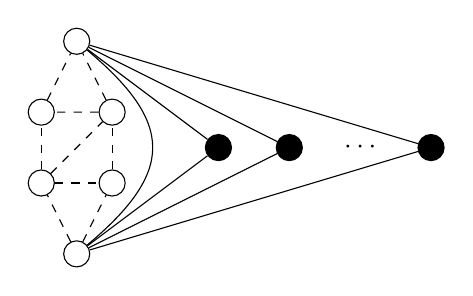
\begin{tikzpicture}[scale=0.9,rotate=90]
    \tikzstyle{w} = [circle, draw, fill=white,
    scale=1.0];
    \tikzstyle{b} = [circle, draw, fill=black,
    scale=1.0];
    \tikzstyle{gd} = [black,dashed,-];

    \node[w] (1) at (0,0){};
    \node[w] (2) at (1,0.5){};
    \node[w] (3) at (1,-0.5){};
    \node[w] (4) at (2,0.5){};
    \node[w] (5) at (2,-0.5){};
    \node[w] (6) at (3,0){};

    \node[b] (7) at (1.5,-2){};
    \node[b] (8) at (1.5,-3){};
    \node[] (9) at (1.5,-4){$\cdots$};
    \node[b] (9) at (1.5,-5){};

    \path[gd] (1) edge (2)
                  edge (3)
              (2) edge (3)
                  edge (4)
                  edge (5)
              (3) edge (5)
              (4) edge (6)
              (5) edge (6)
                  edge (4);
                  
    \path[-]  (1) edge [bend right=50,
                        looseness = 1.5] (6);
    \path[-]  (7) edge (1)
                  edge (6)
              (8) edge (1)
                  edge (6)
              (9) edge (1)
                  edge (6);
                  


  \end{tikzpicture}
    \caption{A problematic graph for algorithm 
    that stores only nodes CPM0.
    It merges dashed and black triangle 
    communities if any 
    black clique is considered after 
    all cliques of the dashed community.
    The number of black cliques
    can be arbitrary large, 
    implying that CPM0 with 
    a random order of clique 
    processing will almost surely merge two 
    communities when the number of black cliques
    tends to infinity.
    Our approximate
    Algorithms~\ref{algo:ckcom2}
    and~\ref{algo:ckcom3} 
    stores links not just nodes. 
    They are immune to this problematic case.
    }
    \label{gr0}
\end{figure}

\begin{figure}
    \centering
  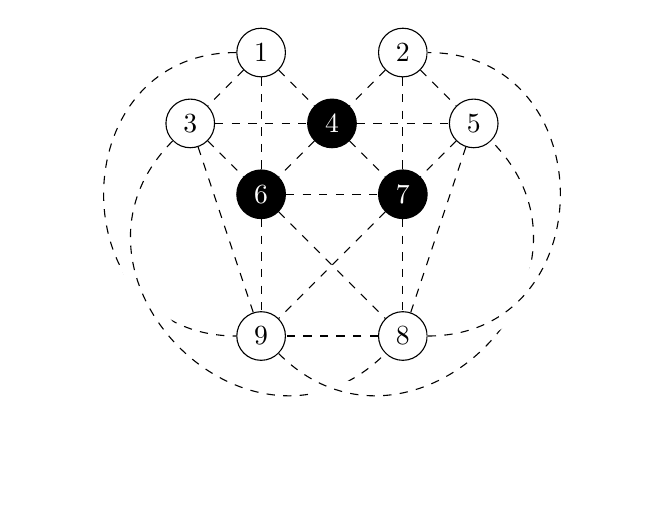
\begin{tikzpicture}[scale=0.9, rotate=0]
   \tikzstyle{nod1} = [circle, draw, fill=black, scale=1.0,
                       text = white];
   \tikzstyle{nod2} = [circle, draw, fill=white, scale=1.0];
   \tikzstyle{gd} = [black,dashed,-];

    \node[nod2] (1) at  (0,0){1};
    \node[nod2] (2) at  (2,0){2};
    
    \node[nod2] (3) at  (-1,-1){3};
    \node[nod1] (4) at  (1,-1){4};
    \node[nod2] (a5) at  (3,-1){5};
    \node[nod1] (a6) at  (0,-2){6};
    \node[nod1] (a7) at  (2,-2){7};
    \node[nod2] (a8) at (2,-4){8};
    \node[nod2] (a9) at (0,-4){9};
    
    \path[gd] (1) edge  (3);
    \path[gd] (1) edge  (4);
    \path[gd] (1) edge  (a6);
    
    \path[gd] (2) edge  (a5);
    \path[gd] (2) edge  (4);
    \path[gd] (2) edge  (a7);
    \path[gd] (3) edge  (4);
    \path[gd] (3) edge  (a6);

    \path[gd] (4) edge  (a6);
    \path[gd] (4) edge  (a7);
    \path[gd] (4) edge  (a5);
    
    \path[gd] (a5) edge  (a7);

    \path[gd] (a6) edge  (a7);
    \path[gd] (a6) edge  (a9);
    \path[gd] (a6) edge  (a8);
    
    \path[gd] (a7) edge  (a9);
    \path[gd] (a7) edge  (a8);


    %% links of a clique from another community
    % \path[thick] (4) edge  (5);
    % \path[thick] (a7) edge  (5);
    % \path[thick] (a6) edge  (5);

    \path[gd] (3) edge (a9);
    \path[gd] (a5) edge (a8);
    
    \path[gd] (1) edge 
    [bend right=90, looseness=1.6] (a9);
    
    \path[gd] (a9) edge 
    [bend right=90, looseness=1.6] (a5);

    \path[white,-] (3) edge 
    [bend right=90, looseness=1.6, line width=3mm
    ] (a8);
    \path[gd] (3) edge 
    [bend right=90, looseness=1.6] (a8);

    \path[white,-] (a9) edge 
    [bend right=90, looseness=1.6, line width=3mm
    ] (a5);
    \path[gd] (a9) edge 
    [bend right=90, looseness=1.6] (a5);

    \path[white,-] (a8) edge
    [bend right=90, looseness=1.6, line width=3mm
    ] (2);
    \path[gd] (a8) edge 
    [bend right=90, looseness=1.6] (2);

    
    \path[gd] (a8) edge  (a9);
    
  \end{tikzpicture}
    \caption{
    A $(k-1)$-clique $F$ is called {\em phantom}
    if it is contained in a (sub)graph covered by a 
    $k$-clique percolation denoted by $P$ but 
    there is no $k$-clique in $P$ that contains $F$.
    %    Alexis Baudin's definition 
    % Etant donné une percolation de 
    % k-cliques sur un graphe, une 
    % communauté est un ensemble de 
    % k-cliques.     Une **(k-1)-clique 
    % parasite** de cette communauté est une
    % (k-1)-clique qui apparait dans le 
    % graphe de la communauté mais qui 
    % n'appartient à aucune clique de la 
    % communauté.
    This figure represents a minimal example
    of a graph covered by a $k$-clique percolation
    and containing a phantom $(k-1)$-clique,
    for $k = 4$. Duplicating a node from the clique
    one can easily generate an additional
    phantom clique.
    }
    \label{gr0}
 \end{figure}



We now proceed to the theoretical analysis of our algorithms.



\subsection{A memory efficient exact algorithm}

A community is a set of $k$-cliques. Keeping in memory all its $k$-cliques, or all its $(k-1)$-cliques, is not scaling well for huge graphs. A way of tackling this issue is to find a way to compress the data. In this section, the main idea is to store a community as a graph, storing only the nodes and the edges of the $k$-cliques added. So, we say that a $k$-clique is in the community if all its nodes and edges are in the community. Consequently, it can happen that a $k$-clique is tested beeing in the community whereas it has not be added to it. So, the community appears to have more $k$-clique that should be. The main issue is that if a $k$-clique appears to be in a community, and is also in another one, the two communities are merged, whereas it should not.

Therefore, whereas keeping the community as a list of edges allows to store communities with few memory, it creates parasites cliques that we need to compute and to store. A $k$-clique is added to the community if it shares a $(k-1)$-clique with it. A $(-1)$-clique parasite of a community is a $(k-1)$-clique that is tested to be in the community but which is not part of any $k$-clique added to the community. In consequence, if the $(k-1)$-clique common to a $k$-clique and a community is a parasite, we need to know it not to add the $k$-clique to the community.

In consequence, we choose to use a procedure to list all the $(k-1)$-cliques parasites of a community. Every time an edge  is added to the community, we list all the $(k-1)$-cliques of the community containing this edge. Each one which is not a sub-clique of the $k$-clique added is then a parasite $(k-1)$-clique (RESULTAT A METTRE EN VALEUR ? + PREUVE ?). Then, we remove all the $(k-1)$-subliques of the $k$-clique added, so the list of $(k-1)$-cliques parasites is always up-to-date.

\begin{algorithm}
  \caption{CPM 3 condensé}
  \begin{algorithmic}[1]
    \State GraphCommus $\gets dict()$ % \Comment{Graphs of communities}
    \State GhostCliques $\gets dict()$ % \Comment{Ghost cliques of communities}
    \State Fusions $\gets []$ % \Comment{Fusions to perform at the end of the algorithm}
    \For{each $k$-clique $c_k \in G$}
    \State commus\_ck $\gets$ \Call{CommusNeighboursOf}{$c_k$, GraphCommus, GhostCliques}
    %\State
    \If{commus\_ck == $\emptyset$} %\Comment{No current community is a neighbour of $c_k$}
    \State \Call{CreateCommu}{$c_k$, GraphCommus, GhostCliques} \Comment{$c_k$ : new community}
    %\State
    \Else \Comment{Pick one neighbour community and add $c_k$ to it, computing new ghost cliques for each new edge}
    \State $commu$ $\gets$ ONE community from commus\_ck
    \State \Call{AddToCommuGraph}{$c_k$, GraphCommus, GhostCliques}
    \If{|commus\_ck| > 1} \Comment{Record the other communities to merge them at the end}
    \State Fusions.push(commus\_ck) 
    \EndIf
    \EndIf
    \EndFor
    %\State 
    \State \Call{ApplyFusions}{Fusions, GraphCommus}
  \end{algorithmic}
\end{algorithm}
\section{Converging algorithms}

\subsection{Lower bound algorithm}



\subsection{Upper bound algorithm}

In this section, we give an algorithm which gives an upper bound of the number of communities from the $k$-clique percolation. This algorithm takes as a parameter the integer $z$ such as $1 \leq z \leq k-1$. The more $z$ is high and the more the algorithm is precise, but with a cost in time and memory efficiency. For $z=k-1$, the value of the bound is the exact number of $k$-clique communities.

The more we add $k$-cliques to a community, the more we increase the possibility of merging it with other communities. So, this upper bound algorithm is based on not adding all the $k$-cliques to the communities (but enough to have a relevant bound). In consequence, some communities which normally have to be merged, are not, and the bound is higher than the real number of $k$-clique communities.

Let $z$ be fixed in $\{1,...,k-1\}$.

A $z$-community is represented as :
\begin{itemize}
\item "Packs" of $k$-cliques added to the community. A pack is the set of $(k-1)$-cliques of the $k$-cliques added. Two types of packs are possible, we need to work out wich one is better :
  \begin{itemize}
  \item a big clique standing for all its $(k-1)$-sublique
  \item the exhaustive list of all $(k-1)$-subliques
  \end{itemize}

  To simplify, we first work on the exhaustive list of all $(k-1)$-subliques added.

\item List of all $z$-subcliques of the $k$-cliques added to the community 
\end{itemize}


\begin{algorithm}[!htbp]
  \caption{One pass over $k$-cliques, storing some $(k-1)$-cliques}
  \begin{algorithmic}[1]
    \State z fixed by the user : $1 \leq z \leq k-1$
    \State $UF \leftarrow$ Union-Find datastructure \Comment{For $(k-1)$-cliques}
    \State $Comz \leftarrow$ List$\{\}$ \Comment{$Comz[p]$ : Set of $z$-cliques of community $p$}
    \For {each $k$-clique $c_k \in G$}
    \State $p\leftarrow NULL$
    \For {each $(k-1)$-clique $c_{k-1}$ in $c_k$}
    \State $q\leftarrow UF.Find(c_{k-1})$
    \If {$p\neq NULL$ {\bf and} $p\neq q$}
    \State $UF.Union(p,q)$
    \State $Comz[q] = Comz[p] \cup Comz[q]$
    \EndIf
    \State $p \leftarrow q$
    \EndFor
    \State $add\_ck \leftarrow False$
    \For {each $z$-clique $c_z$ in $c_k$}
    \If {$c_z \notin Comz[p]$}
    \State $Comz[p].add(c_z)$
    \State $add\_ck \leftarrow True$
    \EndIf
    \EndFor
    \If {$add\_ck$}
    \For {each $(k-1)$-clique $c_{k-1}$ in $c_k$}
    \State $q\leftarrow UF.Find(c_{k-1})$
    \If {$q == NULL$}
    \State $q \leftarrow UF.MakeSet(c_{k-1})$
    \State $UF.Union(p,q)$
    \EndIf
    \EndFor
    \EndIf
    \EndFor
  \end{algorithmic}
\end{algorithm} 

% \input{analysis}
\section{Experimental evaluation}
\label{sec:experiments}

In this section we compare our approach to the state-of-the-art approaches to compute k-clique communities in terms of running time and memory consumption.

\subsection{Experimental Setup}
% and \cite{kunegis2013konect}

We consider several real-world graphs that we obtained from \cite{snapnets} and present in Tables~\ref{tab:net}. These graphs are large having almost one million edges for the smallest one and almost two billion edges for the largest one. They also have ground truth communities, we will use these only in the case study (Section \ref{sec:casestudy}).

\begin{table}
\begin{tabular}{|c|c|c|c|}%|c|c|}
\hline
networks & $n$ & $m$ & $c$ \\%& $k_{max}$ & $N_{k_{max}}$ \\
\hline
\hline
Amazon & \np{334863} & \np{925872} & 7 \\%& 7 & 32\\%&7
Youtube & \np{1134890} & \np{2987624} & 51 \\%& 17 & 2\\%&51
DBLP & \np{425957} & \np{1049866} & 113 \\%& 11 & \num{8.23e14}\\
Orkut  & \np{3072627} & \np{117185083} & 253 \\%& 12 & \num{4.15e14} \\%  \np{415041933452209} \\%
Friendster  & \np{124836180} & \np{1806067135} & 304 \\%& $10$ & \num{4.87e14} \\%& 9h59m32s\\  \np{487090833092739} \\%
LiveJournal & \np{4036538} & \np{34681189} & 360 \\%& $7$& \num{4.49e14} 
\hline
\end{tabular}
\caption{Our set of real-world graphs with ground truth communities.}
\label{tab:net}
\end{table}

% Without this definitions you have some errors
\newcommand{\algo}[1]{Algorithm {#1}}

We carried our experiments on a Linux machine equipped with 4 processors Intel Xeon CPU E5- 2660 @ 2.60 GHz with 10 cores (a total of 40 threads) and with 64 G of RAM DDR4 2133 MHz.\todo{We evaluate both the sequential version of our algorithm, denoted as \algo1, and the parallel version of our algorithm denoted as \algo{$n$}, where $n$ denotes the number of threads. We evaluate our method using 1, 10, and 40 threads (\algo1, \algo10 and \algo{40}, respectively)} against the state-of-the-art for finding k-clique communities\footnote{Our code is available at \url{https://github.com/maxdan94/CPM}.}. In particular, we consider the following approaches:
\begin{itemize}
 \item {\bf Palla et al.:} the algorithm proposed in the original paper introducing CPM \cite{palla2005uncovering}. We used the implementation provided by the authors on the dedicated webpage\footnote{\url{http://www.cfinder.org/}}.
 \item {\bf Kumpula et al.:} The algorithm suggested in \cite{kumpula2008sequential} for which we used ... .
 \item {\bf Reid et al.} The algorithm suggested in \cite{reid2012percolation} ...
 \item {\bf Gregori et al.:} The algorithm suggested in \cite{gregori2013parallel} ...
\end{itemize}
All the state-of-the-art methods except Kumpula et al. use a subroutine that first list all maximal cliques and then compute the $k$-clique communities out of the $k$-cliques. We thus also include the time to list all maximal cliques using the method detailed in \cite{eppstein2011listing} using the implementation provided by the authors. This method is, to the best of our knowledge, the fastest one for sparse real-world graphs. Note that the time bottleneck of this type of approach is actually the second step (building $k$-clique percolated communities out of the maximal cliques) and thus the running time to list all maximal cliques is a -rather not tight- lower bound on the running time. This method will be referred to by {\bf Eppstein et al.}.

%\subsection{Running time and memory consumption}

%Figure~\ref{fig:time} shows the running time of the algorithms as a function of $k$, when executed on our set of graphs. It shows that our sequential algorithm is significantly more efficient than the other approaches, with its running growing more gracefully as a function of $k$. It is at least one two orders of magnitude faster than...

\subsection{Approximation}

{\color{red}

Max, is the following true ?

CPM = Algorithm 1, algorithm gives exact results.

\bigskip

CPM0 is only on github, we store just nodes.
Does CPM0 uses union find or overlapping union find structure ?

\bigskip

CPM1 In overlapping union find we store links, we merge two cliques 
     if they share at least $\frac{(k-1)(k-2)}{2}$ links.
     
\bigskip

CPM2 is Algorithm 3, storing links.

\bigskip

Notations starts to be complicated for me, I propose to adopt CPM0,CPM1,....,CPM(n-1)=CPM

where CPMk stores k-1 cliques
notations.

=============

See also  K-tree  \url{https://en.wikipedia.org/wiki/K-tree}

Our algorithm, that stores links, in fact
detects subgraphs having a spanning K-tree!
Yes it seems to be true but they are not maximal it depends on the order.

In practice we detect something that is between a true k-clique percolation
and a maximal subgraph having spanning k-tree.

It can link and motivate our paper from graph-theoretical perspective
in addition to existing real-world clique-related motivations. And it will be useful to mention such combinatorial construction in the introduction. 

See a graph is connected iff it has a spanning 1-tree.

Our algorithm (that stores links)
detects graph components that are connected in spanning k-tree sense.

Indeed, it is not a clique percolation problem, but k-tree spaning decomposition problem.
We even can define this problem, solve it exactly, than discuss application to clique
percolation.

=========


}
\begin{table}[H]
\begin{tabular}{|c|c|c|c|c|c|}
 \hline
Network & $k$ & \cpm & \cpmA & \cpmBO & \cpmB \\
\hline
\hline
\multirow{4}{*}{Amazon} & 4 & \np{23134} & \np{23111} & \np{23134} & \np{23134}\\
 & 5 & \np{10942} & \np{10942} & \np{10942} & \np{10942}\\
 & 6 & 2621 & 2621 & 2621 & 2621\\
 & 7 & 30 & 30 & 30 & 30\\
\hline
 \multirow{10}{*}{Youtube} & 4 & 7433 & 6840 & 7369 & 7417 \\%7003 & 7270\\
 & 5 & 2606 & 2222 & 2524 & 2575 \\%2261 & 2465\\
 & 6 & 1147 & 872 & 1044 & 1107 \\%882 & 1002\\
 & 7 & 671 & 470 & 591 & 642 \\%461 & 547\\
 & 8 & 346 & 218 & 293 & 322\\%196 & 267\\
 & 9 & 235 & 138 & 192 & 213\\%134 & 176\\
 & 10 & 126 & 96 & 113 & 121\\%88 & 105\\
 & 11 & 71 & 52 & 58 & 67\\
 & 12 & 52 & 35 & 47 & 49\\
 & 13 & 27 & 22 & 26 & 27\\
\hline
 \multirow{3}{*}{DBLP} & 4 & \np{47307} & \np{47025} & \np{47305} & \np{47306}\\% \np{47272} & \np{47289}\\
 & 5 & \np{27075} & \np{27043} & \np{27074} & \np{27075}\\%\np{27062} & \np{27068}\\
 & 6 & \np{14112} & & \np{14112} & \np{14112} \\%\np{14112} & \np{14112}\\
 & 7 & - & & 7388 & 7388 \\%\np{7385} & -\\
\hline
 \multirow{2}{*}{Orkut} & 4 & \np{306755} & \np{115527} & \np{288209} & \np{298676} \\%\np{261277} & \np{282284}\\
  & 5 & - & & \np{227274} & \np{240328} \\%\np{203563} & \np{223128}\\
  & 6 & - & & \np{167610} & \np{179059} \\
\hline
 \multirow{2}{*}{LiveJournal} & 4 & \np{173213} & \np{136591} & \np{170188} & \np{171917} \\%\np{165278} & \np{169256}\\
 & 5 & - & & \np{123470} & \np{125476} \\
\hline
\end{tabular}
\caption{.}
\label{tab:ncoms}
\end{table}

\section{Case Study}
\label{sec:casestudy}

In this section we study the results obtained by our algorithm:
\begin{itemize}
\item Number of k-clique communities and k-clique as a function of k
\item Overlap between the k-clique communities
\item Accuracy compared to the ground truth communities as a function of k.
\end{itemize}






\section{conclusion and discussions}

It works!

However, in some rare cases our approximate Algorithms \ref{algo:ckcom2} and
\ref{algo:ckcom3} merge two different communities into one. 
As we can deduce from real-world experiences,
whose results are presented in Table~\ref{tab:ncoms}, 
it happens only for some rare cases. 
One of such problematic graphs is presented in
Figure~\ref{gr1}. 

{\color{red} VERIFY THIS STATEMENT!}
Algorithms~\ref{algo:ckcom2} and~\ref{algo:ckcom3} 
produce exact results when $k = 3$: because by construction 
they store all $k-1$-cliques, i.e. edges int the case of 
$k=3$.
In order to get around the problematic case illustrated 
on Figure~\ref{gr1}
we could store all triangles. It suggest the creation
of a family of algorithms, the pseudo-code will remain almost
the same, but we replace $E(c_{k-1})$ 
(resp. $E(c_k)$)
by $\mathcal{E}_\ell(c_{k-1})$ (resp. $\mathcal{E}_\ell(c_k)$)
where $\mathcal{E}_\ell(c)$ enumerates all cliques of
size $\ell$ inside a current clique $c$. 
In this regard, our results could be viewed 
as $\ell$-clique relaxation of the original 
clique percolation problem. The quality augments as $\ell$
approaches $k-1$, when $\ell = k-1$ algorithm produces only 
exact results. We could also imagine a sequence of 
passes over the k-cliques considering the difference between 
numbers of detected communities, when this difference is less than $\epsilon$ we say "Ok, it is good enough".

It should be noted, that the order of $k$-clique
processing plays an important yet not fully understood
role in the problematic cases.
It give rise to many interesting
graph theoretical questions about
characterisation of problematic sub-graphs:
how many of them are presented in a typical real-world graph ?
does there exists an order of $k$-clique processing that
completely eliminates all approximation errors ?


{\color{red} 
MAX!!! See, maybe we should turn the paper a way around
and present it as a sequence of approximate algorithms (starting from cpm0) discussing
in more details the sequence of counter-examples and giving some intuitions grown under the light of extensive experiments ? 
Do rare problematic configurations happen
less and less proportionately frequently
when we add more and more value to $\ell$
? 


Doing this we could probably cover
the current lack of serious analysis,
by providing simple formulae based on natural parameters
but extended to $\ell$-clique approximation case.
(A you dare enough to express the complexity using 
parameters that depends on output?)
}

{\color{red} We even could add the last Fantomas example 
from my mail to illustrate how algo CPM0 goes to be bad,
and why cpm1 is better.}

{\color{red}

En fait dans nos communautés il y a des trous...
des zones qui doivent
être interdites
à ajouter les nouveau cliques... 
si jamais on arrive a maintenir
la liste de ces zones de le début ce serait top!
on va gagner ! Car vos expériences montrent que ils sont quand même assez rares.

}

\bibliographystyle{abbrv}
\bibliography{biblio}

\end{document}
